% Alles was im Kopf steht, ausser Funktionsdefinitionen. Diese sollten besser in
% eine eigene Datei ausgelagert werden. Fuer kurze Funktionen einfach in
% functions.tex, sonst ggf. fuer zusammenhaengende Dinge eine eigene Datei.

% Titel, Autor etc. sollten gesetzt werden. Man kann sie bei Bedarf einfach in
% der jeweiligen Praesentation ueberschreiben.

\usepackage[ngerman]{babel}
\usepackage[utf8]{inputenc}
\usepackage[T1]{fontenc}
\usepackage{csquotes}

\usepackage{tikz}
% Für lustige Grafiken
\usetikzlibrary{shapes,snakes,arrows}
\usetikzlibrary{positioning}
\usetikzlibrary{arrows}
\usetikzlibrary{calc,fadings,decorations.pathreplacing}

\usepackage[european]{circuitikz}

\usepackage{pgfplots}
\pgfplotsset{compat=1.11}
\graphicspath{{./images/}}

\usepackage[scaled=.90]{helvet}
\renewcommand\ttdefault{txtt}
\usefonttheme[onlymath]{serif}
\usetheme[footlinenumber, navline=false, footlineauthor]{Bremen}

\fbnum{00}
\fbname{Uni Bremen}
\subject{\LaTeX}

\title{Eine Einführung in \LaTeX{}}
\author[Arbeitsgruppe \LaTeX]{Arbeitsgruppe \LaTeX}
\date{Orientierungswoche \the\year{}}
\institute[Uni Bremen]{Arbeitsgruppe \LaTeX{}\\-- Universität Bremen --}


\makeatletter
\setbeamertemplate{footline}{%
  \usebeamerfont{subsection in head/foot}%
  \mbox{}\rlap{%
    \begin{pgfpicture}{0pt}{0pt}{\paperwidth}{2.8\baselineskip}%
      % Grauer Fond
      \color{coolgray 1}%
      \pgfpathrectangle{\pgfpoint{0cm}{0cm}}{%
	\pgfpoint{\paperwidth}{1.6\baselineskip}}\pgfusepath{fill}
      \pgfpathrectangle{\pgfpoint{0mm}{0cm}}{%
	\pgfpoint{.75\paperwidth}{2.8\baselineskip}}\pgfusepath{fill}
      \color{black}%
      % Universitaetslogo
%      \pgfputat{\pgfpoint{4mm}{1.5\baselineskip}}{%
%	\pgfbox[left,bottom]{\pgfimage[height=2\baselineskip]{unilogo}}%
      %}
    \end{pgfpicture}%
  }
  %% Universitätslogo
  \rlap{%
    \raisebox{.55\baselineskip}{%
      \mbox{}\hspace{4mm}%
      \parbox[b]{.75\paperwidth}{%
	\href{http://www.uni-bremen.de}{%
	  
\includegraphics[height=1.7\baselineskip]{unilogo}}%
	}}}%
  %% Institute/Partnerlogos
  \rlap{%
    \raisebox{1.75\baselineskip}{%
      \mbox{}\hspace{.5\paperwidth}%
      \llap{%
      \parbox[t]{.15\paperwidth}{%
        \vspace{0pt}%
	\mbox{}\hfill%
	\beamer@theme@footline@partnerlogo}%
	\hspace{.025\paperwidth}}
      \rlap{%
      \hspace{.025\paperwidth}%
      \parbox[t]{0.15\paperwidth}{%
        \vspace{0pt}%
	\beamer@theme@footline@secondarypartnerlogo}%
	}}}%
  %% Autor
  \rlap{%
    \raisebox{1.9\baselineskip}{%
      \mbox{}\hspace{.75\paperwidth}%
      \parbox[b]{.25\paperwidth}{%
	\mbox{}\hspace{.5mm}\beamer@theme@footline@author\hfill%
% Ausgelager siehe unten
%	\beamer@theme@footline@number\hfill~\hspace{5mm}
  }}}%
  %%% Foliennummer
  \rlap{%
    \raisebox{1.9\baselineskip}{%
      \mbox{}\hspace{.91\paperwidth}%
      \parbox[b]{.05\paperwidth}{%
        \raggedright\beamer@theme@footline@number
      }
    }
  }
  %% Abschnittsleiste
  \rlap{\raisebox{1.9\baselineskip}{%
      \beamer@theme@footline@section%
  }}%
  %% Navigationssymbole
  \rlap{\parbox[b]{\paperwidth}{%
      \hfill\usebeamertemplate***{navigation symbols lower}%
      \hspace{1.5mm}\mbox{}\vspace{.5mm}%
  }}%
}
\makeatother



\newenvironment{fframe}{\begin{frame}[fragile,environment=specialframe]}{\end{frame}}


\makeatletter
        \providecommand\grpn[1]{\textcolor{OliveGreen}{\texttt{#1}}}
        \providecommand\cls[1]{\textcolor{BurntOrange}{\textsf{#1}}}
        \providecommand\pkg[1]{\cls{#1}}
        \providecommand\umg[1]{\textcolor{SeaGreen!50!Brown}{\texttt{#1}}}
        \providecommand\msur[1]{\texttt{\{#1\}}}
        \providecommand\osur[1]{\texttt{[#1]}}
        \providecommand\meta[1]{\emph{\ensuremath\langle#1\ensuremath\rangle}}
% \cmd{\foo} Prints \foo verbatim
        \def\cmd#1{\cs{\expandafter\cmd@to@cs\string#1}}
        \def\cmd@to@cs#1#2{\char\number`#2\relax}
        \DeclareRobustCommand\cs[1]{\texttt{\char`\\#1}}
% \marg \marg{text} prints {text}, `mandatory argument'.
        \providecommand\marg[1]{%
        {\ttfamily\char`\{}\meta{#1}{\ttfamily\char`\}}}
% \oarg \oarg{text} prints [text], `optional argument'.
        \providecommand\oarg[1]{%
        {\ttfamily[}\meta{#1}{\ttfamily]}}
% \parg \parg{te,xt} prints (te,xt), `picture mode argument'.
        \providecommand\parg[1]{%
        {\ttfamily(}\meta{#1}{\ttfamily)}}

% Keine Abstände vor und nach Codeblöcken
\preto{\@verbatim}{\topsep=1pt \partopsep=1pt }
\makeatother

\newcommand{\uebung}[1]{
\begin{frame}
\frametitle{Zeit zum Ausprobieren}

Die Folien findet ihr hier: \url{\slideurl}

Die Aufgaben hier: \url{\exerciseurl}
\bigskip
\begin{center}
    {\huge
    Bearbeitet jetzt die\\
    Aufgabe #1
    }
\end{center}
\end{frame}}


\renewcommand{\exercisesource}{Die Folien und den Übungszettel findet ihr auf Stud.IP im Ordner \texttt{Latex-Kurs} oder unter \url{http://tinyurl.com/latex-uni-bremen}}

\fbnum{1}
\fbname{Physik / Elektrotechnik}
\institutelogo{
\includegraphics[height=2.5\baselineskip]{images/logo_emodul_physik.png}}
\subtitle{Physik-Edition}

\registerexercise{Uebung-Physik}

\begin{document}

    \begin{frame}
        \frametitle{Wie bekomme ich den Credit Point?}
        \begin{itemize}
            \item Abgabe \emph{eines} der folgenden Dinge bis zum 22.11. beim Mentor:
            \begin{itemize}
                \item Ein in \LaTeX{} erstellter Praktikumsbericht (bspw. zum Probeversuch)
                \item Drei in \LaTeX{} erstellte ausführliche Lösungen von Übungsaufgaben (bspw. aus dem math. Vorkurs.)
            \end{itemize}
            \item Jeweils mit Erläuterung der verwendeten \LaTeX{}-Befehle im Code
            \item Code und Dokument abgeben
        \end{itemize}
        Verbindliche Angaben siehe Stud.IP!
    \end{frame}


    % Alle allgemeinen Folien, zum einfachen einbinden.

\section{\LaTeX{}: Was, warum, wie?}

\begin{frame}
    \frametitle{Texte schreiben im Studium: Was brauchen wir?}
    \begin{itemize}
        \item Text\pause
        \item Abbildungen \& Tabellen\pause
        \item Titelseite\pause
        \item Formeln\pause
        \item Inhaltsverzeichnis\pause
        \item Fußnoten\pause
        \item Quellenangaben
        \item \ldots
    \end{itemize}
\end{frame}

\begin{frame}
    \frametitle{Womit können wir das erreichen?}
    \begin{block}{Mehrere Möglichkeiten mit verschiedenen Ansätzen:}
        \pause	    
	    \begin{itemize}
	        \item LibreOffice
	        \item Word\pause
	        \item \LaTeX
	    \end{itemize}
    \end{block}
\end{frame}

\begin{frame}
    \frametitle{Was ist dieses \LaTeX{}?}
    \LaTeX{} ist
    \begin{itemize}
        \item eine logische Markup-Sprache zur Textauszeichnung\pause
        \item plattformunabhängig und Quelloffen\pause
        \item ideal für wissenschaftliche Dokumente
    \end{itemize}
    \bigskip\pause
    
    \LaTeX{} ist kein
    \begin{itemize}
        \item WYSIWYG\pause
        \item ganz so einsteigerfreundliches Programm
    \end{itemize}
    \medskip\pause
    
    Aber: Das relativiert sich sehr schnell
\end{frame}

\begin{frame}
    \frametitle{Warum also \LaTeX?{}}
    \begin{itemize}
        \item Plattformunabhängig\pause
        \item Hohe typographische Qualität\pause
        \item Gut dokumentiert (Internet, Bücher)\pause
        \item Quasistandard bei wissenschaftlichen Veröffentlichungen\pause
        \item Konzentration auf den Inhalt, nicht das Layout\pause
        \item Zeit- und Stressersparnis
    \end{itemize}
\end{frame}

\begin{frame}
    \frametitle{Was brauchen wir?}
    Unbedingt:
    \begin{itemize}
        \item Eine \LaTeX{}-Distribution, wir benutzen TeX Live\pause
        \item Editor (z.B. Notepad)\pause
        \item PDF-Betrachter
    \end{itemize}
    \pause
    \bigskip
    Besser, ein spezialisierter Editor:
    \begin{itemize}
        \item Texmaker -- Unsere Empfehlung
        \item Kile (KDE)
    \end{itemize}
\end{frame}

\begin{frame}
    \frametitle{So funktioniert \LaTeX{}}
    \begin{itemize}
        \item Übersetzen von geschriebenem Quelltext in PDF-Dokument
        \item Programm dafür: \texttt{pdflatex}
        \item Für erweiterte Funktionen, z.B. Verweise mehrere Durchläufe nötig.
    \end{itemize}
    \pause\bigskip
    \begin{block}{Ablaufschema}\centering
        \begin{tikzpicture}[scale=.75,shorten <=2pt, shorten >=2pt]

            \node[rectangle,label=above:{Code}]
            	(code) 		at (0,0) {
\includegraphics[height=30pt]{texicon.png}};
            \node[rectangle,draw,fill=white]
            	(latex) 	at (3,0) {\texttt{pdflatex}};
            \node[rectangle,label=above:{Dokument}]
            	(dokument) 	at (6,0) {
\includegraphics[height=30pt]{pdficon.png}};
            \node
            	(aux) at (3,-2) {\footnotesize Hilfsdateien: \texttt{.aux}, \texttt{.toc},
            	\texttt{.log}, \ldots};
            \begin{scope}[thick]
                \path[->] (code)  edge (latex);
                \path[->] (latex) edge (dokument);
                \path[<->] (latex) edge (aux);
            \end{scope}
        \end{tikzpicture}
    \end{block}
\end{frame}


\section{Syntax und Grundstruktur}

\begin{frame}[fragile]
    \frametitle{Zur Syntax}
    \begin{block}{Befehl}
        \cmd{Befehl}\oarg{Optionen}\marg{Argument1}...\marg{ArgumentN}
    \end{block}
    \pause
    \begin{block}{Umgebung}
        \cmd{begin}\marg{Umgebung}\oarg{Optionen} \ldots \cmd{end}\marg{Umgebung}
    \end{block}
    \pause
    \begin{block}{Kommentar}
        \verb+% Dies ist ein Kommentar+
    \end{block}
\end{frame}


\begin{frame}[fragile]
    \frametitle{Aufbau der Quelldatei}
    \begin{itemize}
        \item Präambel
        \item \enquote{Inhalt}
    \end{itemize}
    \bigskip
    \pause
    
    \begin{block}{\texttt{Beispiel.tex}}
\begin{verbatim}
\documentclass{scrartcl}
% Ende der Präambel

\begin{document}
    Hallo Welt
\end{document}
\end{verbatim}
    \end{block}
\end{frame}


\begin{frame}[fragile]
    \frametitle{Was kommt wo hin?}
    Präambel (Header)
    \begin{itemize}
        \item Dokumentenklasse
        \item Benutzte Pakete
        \item Einstellungen für das gesamte Dokument
        \item Einige Metadaten, z.B. Autor, Titel, \ldots
    \end{itemize}
    \bigskip

    Der eigentliche Inhalt (Text, Abbildungen, \ldots) kommt zwischen \verb+\begin{document}+ und \verb+\end{document}+
\end{frame}


\begin{frame}[fragile]
    \frametitle{Die Dokumentenklasse}
    \begin{block}{Syntax}
        \cmd{documentclass}\oarg{Optionen}\marg{Klasse}
    \end{block}
    \pause
    \begin{itemize}
        \item Dokumentklassen
        \begin{itemize}
            \item Die wichtigste Klasse: \verb+scrartcl+\pause
            \item Weitere: \verb+scrreprt+, \verb+scrbook+, \verb+scrlttr2+, \verb+beamer+\pause
        \end{itemize}
        \item Optionen:
        \begin{itemize}
            \item Schriftgröße: \verb+10pt+, \verb+11pt+, \verb+12pt+\pause
            \item Papiergröße: \verb+a4paper+\pause
            \item Zweispaltig: \verb+twocolumn+\pause
            \item Keine Einrückung am Anfang vom Absatz: \verb+parskip=full+
        \end{itemize}
    \end{itemize}
\end{frame}


\begin{frame}
    \frametitle{Die Dokumentenklassen im Überblick}

    \begin{tabular}{l|c|c}
        Dokumenttyp & KOMA-Klasse & Standard-Klasse\\
        \hline
        Einfacher Artikel & scrartcl & article\\
        längerer Report & scrreprt & report\\
        Buch & scrbook & book\\
        Briefe & scrlttr2 & --
    \end{tabular}
    
    \bigskip
    
    In der Regel sind die KOMA-Klassen den Standard-Klassen vorzuziehen, da die KOMA-Klassen an die deutsche Formatierung angepasst sind.
\end{frame}


\begin{frame}[fragile]
    \frametitle{Pakete einbinden}
    
    Latex kann mit Paketen erweitert werden. Dies ist für viele Dinge sehr wichtig, da die Standardfunktionen zum Teil nicht ausreichen.
    \begin{block}{Paket mit Optionen laden}
        \cmd{usepackage}\oarg{Optionen}\marg{Paketname}
    \end{block}
    \pause
    \bigskip
    \begin{exampleblock}{Quelldatei ist UTF-8, immer nutzen}
		\verb+\usepackage[utf8]{inputenc}+
    \end{exampleblock}
    \pause
    \begin{exampleblock}{Sprache auf Deutsch umstellen}
        \verb+\usepackage[ngerman]{babel}+
    \end{exampleblock}
\end{frame}


\begin{frame}[fragile]
    \frametitle{Das babel-Paket}
    
    Sehr wichtiges Paket zur Lokalisierung:
    \begin{itemize}
        \item Deutsche Überschriften für z.B. Verzeichnisse
        \item Deutsche Silbentrennung
        \item Deutsche Anführungszeichen
    \end{itemize}
    \bigskip
    \begin{block}{Benutzen mit}
        \verb+\usepackage[ngerman]{babel}+
    \end{block}
\end{frame}


\begin{frame}[fragile]
    \frametitle{Umlaute}
    
    Umlaute funktionieren nicht Standardmäßig, Latex muss gesagt werden wie die Datei gespeichert ist:
    \begin{block}{Quelldatei ist UTF-8}
		\verb+\usepackage[utf8]{inputenc}+
    \end{block}
    \pause
    
    Eventuell muss Latex außerdem eine andere Schrift zur Ausgabe nutzen:
    \begin{block}{Andere Font-Darstellung}
		\verb+\usepackage[T1]{fontenc}+
    \end{block}
\end{frame}


\begin{frame}[fragile]
    \frametitle{Sonderzeichen}
    
    Latex nutzt die folgenden Sonderzeichen für spezielle Funktionen:
    \begin{center}
      \hfill \$
      \hfill \%
      \hfill \&
      \hfill \{
      \hfill \}
      \hfill \_
      \hfill \#
      \hfill \textbackslash
      \hfill \~{}
      \hfill \^{}
      \hfill
    \end{center}

    Um diese auszugeben, muss meist nur ein \textbackslash{} vor dieses gesetzt werden.
    Damit wird \verb+\$+ zu \$.
\end{frame}


\begin{frame}[fragile]
    \frametitle{Leerzeichen und Absätze}
    
    \begin{itemize}
        \item Mehrere Leerzeichen werden zu einem zusammengefasst \pause
        \item Ein neuer Absatz mit einer Leerzeile \pause
        \item Einen harten Umbruch erzeugt man mit \textbackslash\textbackslash
    \end{itemize}
    \pause    
    
    \begin{columns}[c]
        \column{.5\textwidth}
            \begin{verbatim*}
Dies ist ein Text  mit
vielen   Leerzeichen, die
verschwinden.
Und eine neue  Zeile.

Ein neuer Absatz geht auch!
\end{verbatim*}
        \pause
        \column{.5\textwidth}
        Dies ist ein Text  mit
        vielen   Leerzeichen, die
        verschwinden.
        Und eine neue  Zeile.

        Ein neuer Absatz geht auch!
\end{columns}
\end{frame}

\section{Das erste Dokument}

\begin{frame}
    \frametitle{Los geht's!}
    \begin{itemize}
        \item Einen Ordner für diese Einführung anlegen
        \item Texmaker starten
        \item Den Texmaker auf UTF-8 umstellen
        \item Die Datei in diesem Ordner mit Namen \texttt{Beispiel.tex} abspeichern
    \end{itemize}
\end{frame}


\begin{frame}[fragile]
    \frametitle{Unser erstes Dokument}
    \begin{codeblock}[Beispiel.tex]
    \begin{verbatim}
\documentclass{scrartcl}

\begin{document}
    Hallo Welt
\end{document}
\end{verbatim}
    \end{codeblock}
\end{frame}


\begin{frame}[fragile]
    \frametitle{Das PDF erstellen}
    \begin{block}{Im Texmaker}
        \begin{itemize}
            \item Klick auf den Pfeil links neben \enquote{Schnelles Übersetzen}
            \item Die Taste F1 auf der Tastatur drücken
            \item Über das Menü \enquote{Werkzeuge}
        \end{itemize}
    \end{block}\pause
    
    \bigskip
    \begin{block}{Alternativ im Terminal}
        \verb+pdflatex Beispiel.tex+
    \end{block}
\end{frame}


\begin{frame}
    \frametitle{Hilfe! Da ist alles Rot!}
    \begin{alertblock}{Wenn es doch nicht geht}
	    \begin{itemize}
	        \item Lest die Fehlermeldungen!\pause
	        \item \texttt{undefined control sequence} heißt: Den Befehl gibt es
	            nicht. Ihr habt ihn entweder falsch geschrieben oder ein
	            benötigtes Paket vergessen\pause
	        \item \texttt{missing \$ inserted} heißt: Ihr habt Befehle aus dem
	            Mathemodus benutzt, ohne in diesen zu wechseln. Oder ihn
	            vergessen zu beenden.
	    \end{itemize}
    \end{alertblock}
\end{frame}


\begin{frame}
    \frametitle{Hilfe zur Selbsthilfe}
    Wenn ihr den Fehler einfach nicht findet oder auch ein Problem nicht lösen könnt, versucht etwas von dem Folgenden:
    \begin{itemize}
        \item Mentor / Betreuer aus der Einführungswoche fragen
        \item Kommilitonen fragen
        \item Im Internet nach der Lösung suchen.
    \end{itemize}
    
    \bigskip
    Im Internet findet man außerdem sämtliche Handbücher.
\end{frame}

\uebung{1.1 bis 1.4}
\begin{loesung}
    \frametitle{Was passiert ohne \pkg{inputenc}}

    \begin{itemize}
        \item Ohne \pkg{inputenc} gehen die Umlaute nicht
        \item Mit \texttt{latin1} als Option gehen sie auch nicht \pause
        \item[\textrightarrow] Die Einstellung im Editor muss die selbe sein wie im Dokument
    \end{itemize}
    
    \bigskip
    Im Texmaker: Anzeige der Kodierung unten rechts in der Leiste.\\
    Man kann das unter \enquote{Optionen \textrightarrow{} Texmaker konfigurieren \textrightarrow{} Editor} ändern, es sollte immer auf UTF-8 stehen.
\end{loesung}

\begin{loesung}
    \frametitle{Wie setzt man \textbackslash{} und \^{}Hallo?}
    
    \begin{itemize}
        \item \textbackslash{} ist das einzige Zeichen, wo ein \textbackslash{}
            davor nicht zum gewünschten Ergebnis führt
        \item[\textrightarrow] Eigener Befehl: \cmd{textbackslash}\pause
        \medskip
        \item Das Dach funktioniert wie es soll, ergibt aber \^ Hallo
        \item[\textrightarrow] Damit das Zeichen davor bleibt, muss \cmd{\^{}\{\}}
            benutzt werden.\pause
        \medskip
        \item[\textrightarrow] Dies ist auch beim Backslash sinnvoll, da das
            nachfolgende Leerzeichen sonst verschwindet
    \end{itemize}
\end{loesung}

\section{Markup und Layout}

\begin{frame}[fragile]
    \frametitle{Absätze und Umbrüche}
    
    Um einen neuen Absatz anzufangen, muss eine Leerzeile eingefügt werden
    
    \bigskip
    Einen normalen Umbruch erhält man mit \texttt{\textbackslash\textbackslash}
    
    \bigskip
    Für eine neue Seite bzw. Spalte gibt es den Befehl \verb+\newpage+\\
    Alternativ: \verb+\clearpage+ beginnt immer eine neue Seite
    
    \bigskip
    Um den Abstand zwischen den Absätzen zu vergrößern, kann an der Stelle einer der folgenden Befehle verwendet werden: \verb+\smallskip+, \verb+\medskip+, \verb+\bigskip+
\end{frame}


\begin{frame}
    \frametitle{Das Dokument gliedern}
    Um das Dokument zu teilen, können wir verschiedene Überschriften definieren:
    \medskip
    \begin{center}
        \begin{tabular}{ll}
            \textbf{Befehl} & \textbf{Verwendung}\\
            \cmd{part}\marg{Name} & Bücher\\
            \cmd{chapter}\marg{Name} & Reports, Bücher\\
            \cmd{section}\marg{Name} & Alle\\
            \cmd{subsection}\marg{Name} & Alle\\
            \cmd{subsubsection}\marg{Name} & Alle\\
            \cmd{paragraph}\marg{Name} & Alle\\
            \cmd{subparagraph}\marg{Name} & Alle
        \end{tabular}
    \end{center}
    \medskip
    In Artikeln (\texttt{scrartcl}) werden meist nur die sections verwendet.
\end{frame}


\begin{frame}[fragile]
    \frametitle{Hervorhebungen im Text}
    
    Um Textstellen hervorzuheben, bietet \LaTeX{} einige Varianten:
    \medskip
    \begin{center}
        \begin{tabular}{ll}
            \textbf{Befehl} & \textbf{Ergebnis}\\
            \verb+\emph{Text}+ & \emph{Text}\\
            \verb+\textbf{Text}+ & \textbf{Text}\\
            \verb+\textit{Text}+ & \textit{Text}\\
            \verb+\underline{Text}+ & \underline{Text}\\
            \verb+\texttt{Text}+ & \texttt{Text}
        \end{tabular}
    \end{center}
\end{frame}


\begin{frame}[fragile]
    \frametitle{Inhaltsverzeichnis}
    Ein Inhaltsverzeichnis ist einfach mit \verb+\tableofcontents+ zu erhalten. Hierzu werden alle Überschriften verwendet.
    \medskip    
    
    Überschriften ohne Nummer und Eintrag im Inhalt erstellt man mit der gesternten Variante, z.B. \cmd{section}*\marg{Name}.
    
    \medskip
    Genauso kann man Verzeichnisse von Tabellen und Abbildungen erzeugen. Dazu später mehr.
    
    \medskip
    \begin{alertblock}{Achtung}
        Für Verzeichnisse benötigt \LaTeX{} einen zweiten Aufruf, nach dem ersten ist das Inhaltsverzeichnis noch leer.
    
        \smallskip
        Dies gilt auch für Änderungen an den Überschriften.
    \end{alertblock}
\end{frame}


\begin{frame}[fragile]
    \frametitle{Der Titel}
    
    \LaTeX{} kann den Titel automatisch setzen, dafür müssen aber die entsprechenden Angaben in der Präambel gemacht werden:
    \medskip
    \begin{center}
        \begin{tabular}{ll}
            \cmd{title}\marg{Name} & Setzt den Titel*\\
            \cmd{author}\marg{Name} & Setzt den Autor*\\
            \cmd{date}\marg{Datum} & Setzt das Datum\\
            \cmd{subtitle}\marg{Name} & Setzt den Untertitel\\
            \cmd{publisher}\marg{Name} & Setzt den Herausgeber
        \end{tabular}
    \end{center}
    \medskip
    Angaben mit einem Stern sind Pflicht.
    \medskip
    
    
    Der Titel wird nun im Dokument mit \verb+\maketitle+ erstellt.
\end{frame}


\begin{frame}
    \frametitle{Umgebungen}
    \LaTeX{} steuert viele Dinge über Umgebungen.\\
    Eine Umgebung wird mit
    \begin{center}
        \cmd{begin}\marg{Name}
    \end{center}
    gestartet und mit
    \begin{center}
        \cmd{end}\marg{Name}
    \end{center}
    wieder beendet.
    
    \bigskip
    Ihr kennt bereits die \texttt{document}-Umgebung
\end{frame}


\begin{frame}[fragile]
    \frametitle{Textausrichtung}
    \framesubtitle{Zentriert mittels \umg{center}}

    \begin{center}
        \fbox{\begin{minipage}{0.7\linewidth}
            \begin{center}
                Text (und mehr) lässt sich mit der \umg{center}-Umgebung
                zentrieren, wenn gewünscht.
            \end{center}
        \end{minipage}}
    \end{center}
    
    \begin{center}
        \begin{verbatim}
        \begin{center}
            Text (und mehr) lässt sich
            mit der center-Umgebung
            zentrieren, wenn gewünscht.
        \end{center}
        \end{verbatim}
    \end{center}
\end{frame}


\begin{frame}[fragile]
    \frametitle{Textausrichtung}
    \framesubtitle{Linksbündig mittels \umg{flushleft}}

    \begin{center}
        \fbox{\begin{minipage}{0.7\linewidth}
            \begin{flushleft}
                Standardmäßig benutzt \LaTeX{} Blocksatz. Wenn stattdessen ein linksbündiger Flattersatz verwendet werden soll, ist das natürlich auch möglich. Hierzu gibt es die \umg{flushleft}-Umgebung.
            \end{flushleft}
        \end{minipage}}
    \end{center}
    
    \begin{center}
        \begin{verbatim}
        \begin{flushleft}
            Standardmäßig benutzt \LaTeX{} Blocksatz.
            Wenn stattdessen ein linksbündiger
            Flattersatz verwendet werden soll...
        \end{flushleft}
        \end{verbatim}
    \end{center}
\end{frame}


\begin{frame}
    \frametitle{Aufzählungen und Listen}

    Aufzählungen sind ebenfalls Umgebungen.\\
    Dies bedeutet
    \begin{itemize}
        \item Man kann sie Schachteln
        \item Sie haben eine einfache Syntax
    \end{itemize}
    
    \bigskip
    \LaTeX{} bietet die folgenden Umgebungen:
    \begin{itemize}
        \item \umg{itemize} erzeugt Bullets wie in dieser Liste
        \item \umg{enumerate} erzeugt nummerierte Aufzählungen
        \item \umg{description} erzeugt Erläuterungen
    \end{itemize}
\end{frame}


\begin{frame}[fragile]
    \frametitle{Aufzählungen und Listen}
    \framesubtitle{Ungeordnete Listen mit \umg{itemize}}
    
    Eine Aufzählung sieht so aus:
    \begin{itemize}
        \item Erster Eintrag
        \item Letzter Eintrag
    \end{itemize}
    
    \bigskip
    \begin{verbatim}
Eine Aufzählung sieht so aus:
\begin{itemize}
    \item Erster Eintrag
    \item Letzter Eintrag
\end{itemize}
    \end{verbatim}
\end{frame}


\begin{frame}[fragile]
    \frametitle{Aufzählungen und Listen}
    \framesubtitle{Ungeordnete Listen mit \umg{itemize}}
    
    Schachtelung ist auch möglich
    \begin{itemize}
        \item Erster Eintrag
        \begin{itemize}
            \item Unterpunkt
            \item anderer Unterpunkt
        \end{itemize}
        \item Letzter Eintrag
    \end{itemize}
    
    \smallskip
    \begin{verbatim}
Eine Aufzählung sieht so aus:
\begin{itemize}
    \item Erster Eintrag
    \begin{itemize}
        \item Unterpunkt
        \item anderer Unterpunkt
    \end{itemize}
    \item Letzter Eintrag
\end{itemize}
    \end{verbatim}
\end{frame}


\begin{frame}[fragile]
    \frametitle{Aufzählungen und Listen}
    \framesubtitle{Geordnete Listen mit \umg{enumerate}}
    
    Eine Aufzählung sieht so aus:
    \begin{enumerate}
        \item Erster Eintrag
        \item Letzter Eintrag
    \end{enumerate}
    
    \bigskip
    \begin{verbatim}
Eine Aufzählung sieht so aus:
\begin{enumerate}
    \item Erster Eintrag
    \item Letzter Eintrag
\end{enumerate}
    \end{verbatim}
    \medskip
    
    Eine andere Umgebung, der Rest ist gleich
\end{frame}


\begin{frame}[fragile]
    \frametitle{Aufzählungen und Listen}
    \framesubtitle{Beschreibungen mit \umg{description}}
    
    Mit der \umg{description}-Umgebung kann man Erläuterungen erzeugen
    \medskip
    \begin{description}
        \item[\LaTeX{}] Ist ein tolles Programm zum Textsatz welches anfangs komplizierter ist, nachher aber viele Probleme vereinfacht
        \item[MS Word] Kann auch viel, nur nicht so schön
    \end{description}
    
    \bigskip
    \begin{verbatim}
\begin{description}
    \item[\LaTeX{}] Ist ein tolles Programm zum Textsatz
    \item[Microsoft Word] Kann auch viel, ...
\end{description}
    \end{verbatim}
\end{frame}


\begin{frame}[fragile]
    \frametitle{Zitate}
    \framesubtitle{Die \umg{quote}-Umgebung}
    
    Zitate können mit der \umg{quote}-Umgebung sehr einfach vom restlichen Text abgehoben werden:
    \begin{quote}
        Seht mich an, ein Gehirn von der Größe eines Planeten, und man verlangt von mir,
        euch in die Kommandozentrale zu bringen. Nennt man das vielleicht berufliche
        Erfüllung? Ich jedenfalls tu's nicht.
    \end{quote}
    
    \bigskip
    \begin{verbatim}
\begin{quote}
    Seht mich an, ...
\end{quote}
    \end{verbatim}
\end{frame}


\begin{frame}[fragile]
    \frametitle{Quelltexte mit \umg{verbatim}}
    
    Quelltext kann mit der \umg{verbatim}-Umgebung gesetzt werden:
    
    \medskip
    \begin{verbatim}
Mit \LaTeX{} kann man tolle Sachen machen.
    \end{verbatim}
    
    \pause
    \begin{semiverbatim}
\\begin\{verbatim\}
Mit \\LaTeX\{\} kann man tolle Sachen machen.
\\end\{verbatim\}
    \end{semiverbatim}
    
    \begin{alertblock}{Achtung}
        Es werden keine Zeilen mehr umgebrochen, alle Leerzeichen werden so abgedruckt wie im Quelltext. Bessere Quelltextdarstellung z.B. mit dem Paket \pkg{listings}
    \end{alertblock}
\end{frame}


\begin{frame}[fragile]
    \frametitle{Verweise im Dokument}
    \begin{alertblock}{Problem}
        Man will auf ein Kapitel verweisen: \verb+siehe Kapitel 3+.\pause
        
        Nun fügt man ein neues Kapitel vor diesem ein und alle Verweise stimmen nicht mehr.
    \end{alertblock}
    
    \pause
    \begin{block}{Lösung: Labels und Verweise}
        \begin{itemize}
            \item Man kann an vielen Stellen mit \cmd{label}\marg{Bezeichnung} ein Label setzen
            \item Man bekommt die Nummer des Kapitels, des Eintrags in einer \umg{enumerate}-Umgebung etc. nun mit \cmd{ref}\marg{Bezeichnung}
        \end{itemize}
    \end{block}
\end{frame}

\begin{frame}[fragile]
    \frametitle{Verweise im Dokument}
    \framesubtitle{Ein Beispiel}
    Ein Label kann zum Beispiel an eine Überschrift vergeben werden. Dann kann mit \cmd{ref} die Kapitelnummer und mit \cmd{pageref}\marg{Bezeichner} die Seitenzahl benutzt werden:
    \bigskip
    \pause

    \begin{verbatim}
\section{Test}\label{sec:Test}
In Kapitel \ref{sec:Test} auf Seite \pageref{sec:Test}
    \end{verbatim}
    
    \pause
    \begin{alertblock}{Achtung}
        So wie Verzeichnisse brauchen auch Verweise zwei Durchläufe von \LaTeX{}, sonst werden nur zwei Fragezeichen angezeigt!
    \end{alertblock}
\end{frame}


\begin{frame}[fragile]
    \frametitle{Tipps und Tricks}
    \framesubtitle{Worttrennungen}
    Manchmal sind die automatischen Worttrennungen oder Zeilenumbrüche unpassend.
    \medskip    
    
    Diese können mit einem geschützten Leerzeichen (\texttt{\~{}}) verhindert werden: \verb+Am 9.~September+ $\Rightarrow$ Am 9.~September
    
    \medskip
    Außerdem ist es möglich, die Silbentrennung für einzelne Wörter anzupassen, wenn die automatische Trennung falsch ist.
    
    Beispiel: \verb+Staats\-ver\-trag+ wird nur an den markierten Stellen getrennt.
\end{frame}

\uebung{1.5 bis 1.15}
    \uebung{markuplayout}
    \section{Mathematik-Modus}
\subsection{Umgebungen}
\begin{frame}[fragile]{Mathematische Grundlagen}
\framesubtitle{Das Paket \pkg{amsmath}}
Wir wollen nun erläutern, wie man in \LaTeX{} Formeln schreibt.

\medskip\pause
Wir laden das Paket \pkg{amsmath} durch \verb+\usepackage{amsmath}+. Mit diesem haben wir nun Zugriff auf eine Vielzahl mathematischer Befehle.

\medskip\pause
Formeln sehen anders aus, als der normale Textmodus (z.B. Bindestrich vs. Minus), deshalb müssen wir in \LaTeX{} erstmal den Mathe-Modus aktivieren.

\medskip\pause
Dafür gibt es verschiedene Möglichkeiten. Im Fließtext verwendet man typischerweise Dollarzeichen: \$ \emph{kurze Formel} \$

Einzeilige abgesetzte Formeln werden in eckigen Klammern geschrieben: 
\begin{center}
\textbackslash[\emph{Lange oder hervorgehobene Formel} \textbackslash]
\end{center}
\end{frame}

\begin{frame}[fragile]{Math. Grundlagen Beispiele}
\begin{columns}
\begin{column}{.48\textwidth}\footnotesize
\begin{codeblock}
\begin{verbatim}
	Text mit $a^2=\frac{1}{2}$
	Formel drin.

	Abgesetzte Formel:
	\[a^2=\frac{1}{2}\]
	Text nach der abgesetzten
	Formel.
\end{verbatim}
\end{codeblock}
\end{column}
%
\begin{column}{.45\textwidth}	\pause	
	Text mit $a^2=\frac{1}{2}$ Formel drin.
    
    \pause
	Abgesetzte Mathematik:
	\[a^2=\frac{1}{2}\]
	Text nach der abgesetzten Formel.
\end{column}
\end{columns}
\end{frame}






\begin{frame}[fragile]{Weitere Mathematik}
Formeln durchnummerieren mit Umgebungen. 

\pause
\begin{itemize}
\item \umg{equation}: Nummeriert einzeilig;\pause
\item \umg{align}: Nummeriert mehrzeilig;\pause
\item \umg{alignat}\textrm{\{\textlangle Spaltenzahl\textrangle\}}: Nummeriert mehrzeilig mit festerSpaltenzahl.\pause
\item \umg{equation*}: Ohne Nummerierung einzeilig;
\item \umg{align*}: Ohne Nummerierung mehrzeilig;
\item \umg{alignat*}\textrm{\{\textlangle Spaltenzahl\textrangle\}}: Ohne Nummerierung mit fester Spaltenzahl.
\end{itemize}
\end{frame}

\begin{frame}[fragile]{Beispiele}
\begin{columns}
\begin{column}{.48\textwidth}\footnotesize
\begin{codeblock}
\begin{verbatim}
	Abgesetzt, nummeriert, 
	einzeilig:
    \begin{equation}
    a^2+b^2=c^2
    \end{equation}
    Abgesetzt, nummeriert,
     mehrzeilig:
    \begin{align}
    i^{2} = (-1)\\
    \exp{(i\pi)} = (-1) 
    \end{align}
\end{verbatim}
\end{codeblock}
\end{column}
%
\begin{column}{.45\textwidth}	\pause	
	Abgesetzt, nummeriert, einzeilig:
    \begin{equation}
    a^2+b^2=c^2
    \end{equation}\pause
    Abgesetzt, nummeriert, mehrzeilig:
    \begin{align}
    i^{2} = (-1)\\
    \exp{(i\pi)} = (-1) 
    \end{align}
\end{column}
\end{columns}
\end{frame}
\begin{frame}[fragile]{Die \umg{alignat}-Umgebung}
\framesubtitle{Aussehen} 
Die \umg{alignat}-Umgebung empfiehlt sich vor allem bei Umformen von Gleichungen. Ein Beispiel:
\begin{columns}
\begin{column}{.5\textwidth}
\begin{codeblock}
\begin{verbatim}
\begin{alignat}{2}
&& a &= b + c\\
\iff \quad && a - c &= b\\
\iff \quad && c &= a - b
\end{alignat}
\end{verbatim}
\end{codeblock}
\end{column}

\begin{column}{.4\textwidth}
Wir erhalten:
\begin{alignat}{2}
&& a &= b + c\\
\iff \quad && a - c &= b\\
\iff \quad && c &= a - b
\end{alignat}
\end{column}
\end{columns}
\pause
Beachte: \alert{Am ende der letzten Zeile darf kein \textbackslash\textbackslash{} stehen!}
\end{frame}

\begin{frame}[fragile]{Die \umg{alignat}-Umgebung}
\framesubtitle{Aussehen}
Betrachten wir nun folgendes Beispiel: 

\begin{codeblock}
\begin{verbatim}
\begin{alignat}{4}
a + (3 + 1) &= a + 4          &=&a + (2 + 2)\\
            &= a + (0 + 4)    &=&a + (-1 + 5)\\
b + 102     &= b + 100        &=&b + (49 + 51)\\
            &= b + 1000 - 900 &=&b + (49 + 51)
\end{alignat}
\end{verbatim}
\end{codeblock}
\end{frame}

\begin{frame}{Die \umg{alignat}-Umgebung}
\framesubtitle{Aussehen}
\begin{alignat}{4}
a + (3 + 1) &= a + 4          &=&a + (2 + 2)\\
            &= a + (0 + 4)    &=&a + (-1 + 5)\\
b + 102     &= b + 100        &=&b + (49 + 51)\\
            &= b + 1000 - 900 &=&b + (49 + 51)
\end{alignat}
Was fällt auf?

\medskip
\pause
Die \umg{alignat}-Umgebung wechselt stets zwischen rechts-links-Ausrichtung.
\end{frame}

\begin{frame}[fragile]{Die \umg{alignat}-Umgebung}
Problem: Eine Zeile aus einer \umg{alignat}-Umgebung soll nicht nummeriert werden, bzw. wir wollen eine Zeile anders nummerieren.

\medskip\pause
Lösung: Die Befehle \cmd{notag} und \cmd{tag}\marg{Text}.

\begin{columns}
\begin{column}{0.5\textwidth}
\begin{codeblock}
\begin{tiny}
\begin{verbatim}
\begin{alignat}{2}
 x^2 &=1 \\
 a^2 + b^2 &= c^2 \notag\\ 
 i\hbar \frac{\partial}{\partial t}|\psi(t)
 \rangle&=\mathbb{H}|\psi(t)\rangle \tag{S}
\end{alignat}
\end{verbatim}
\end{tiny}
\end{codeblock}
\end{column}
\begin{column}{0.45\textwidth}
\begin{alignat}{2}
 x^2 &=1 \\
 a^2 + b^2 &= c^2 \notag\\ 
 i\hbar \frac{\partial}{\partial t}|\psi(t)\rangle&=\mathbb{H}|\psi(t)\rangle \tag{S}
\end{alignat}
\end{column}
\end{columns}

\medskip\pause
Mit dem Befehl \cmd{tag}\marg{Text} lässt sich in der \umg{alignat*}-Umgebung auch eine einzelne Gleichung nummerieren. 
\end{frame}

\subsection{Wie nutzt man Mathe}

\begin{frame}[fragile]{Wie mache ich Mathe?}
Wir wissen nun, wo wir Mathematik hinschreiben, aber noch nicht wirklich wie.
\begin{columns}
\begin{column}{0.55\textwidth}
\begin{codeblock}
\begin{verbatim}
Hochgestellt $a^{hoch}$ 
 vs. $a^bc$
Index $a_{Index}$ 
 vs. $a_bc$
Summe $\sum$, Integral $\int$
Grenzen $\sum_a^b$ 
 vs. $\displaystyle\sum_a^b$
Gr. Buchstaben $\alpha, \beta$
\end{verbatim}
\end{codeblock}
\end{column}
\pause
\begin{column}{0.4\textwidth}
Hochgestellt $a^{hoch}$ vs. $a^bc$. 

\medskip\pause
Index $a_{Index}$ vs. $a_bc$.

\medskip\pause
Summe $\sum$, Integral $\int$.

\medskip\pause
Grenzen $\sum_a^b$ vs. $\displaystyle \sum_a^b$

\medskip\pause
Gr. Buchstaben $\alpha, \beta$.
\end{column}
\end{columns}
\end{frame}


\begin{frame}[fragile]{Wie mache ich Mathe II}
\begin{columns}
\begin{column}{0.55\textwidth}
\begin{codeblock}
\begin{verbatim}
Physikalische Ableitungen 
 $\dot{x}$ und $\ddot{x}$. 
Vektoren $\vec{a}$.
Ableitungsoperator $\partial$.
\end{verbatim}
\end{codeblock}
\end{column}
\pause
\begin{column}{0.4\textwidth}
Physikalische Ableitungen $\dot{x}$ und $\ddot{x}$. 

\medskip\pause
Vektoren $\vec{a}$.

\medskip\pause
Ableitungsoperator $\partial$.
\end{column}
\end{columns}
\end{frame}

\begin{frame}[fragile]{Brüche}
Für Brüche benötigt man in \LaTeX{} weder Sonderzeichen, noch diverse andere Methoden. Brüche heißen im Englischen \glqq fraction\grqq{} und auf naive Weise erhält man durch den Befehl
\begin{center}
\cmd{frac}\marg{Zähler}\marg{Nenner}
\end{center}
einen Bruch im Mathe-Modus:
\begin{columns}
\begin{column}{0.55\textwidth}
\begin{codeblock}
\begin{verbatim}
\frac{\exp(i\pi)}{i^2} = 1
\end{verbatim}
\end{codeblock}
\end{column}
\begin{column}{0.35\textwidth}
Das Ergebnis sieht dann so aus:
\[
    \frac{\exp(i\pi)}{i^2} = 1
\]
\end{column}
\end{columns}
\end{frame}


\begin{frame}[fragile]{Abstände in \LaTeX}
\LaTeX{} ignoriert Leerzeichen im Mathemodus. Wir können aber durch bestimmte Befehle Leerzeichen hinzufügen.\pause
\begin{center}
\begin{tabular}{p{0.2\textwidth}p{0.6\textwidth}}
Befehl & Bedeutung\\
\verb+\,+ & Setzt ein Leerzeichen. \\
\verb+\quad+ & Setzt einen Abstand von 1em. \\
\verb+\qquad+ & Setzt einen Abstand von 2em.
\end{tabular}
\end{center}\pause
\begin{columns}
\begin{column}{0.4\textwidth}
\begin{codeblock}
\begin{verbatim}
a\,b\quad c \qquad d
\end{verbatim}
\end{codeblock}
\end{column}
\begin{column}{0.35\textwidth}
Beachte größer werdende Abstände: 
\[
a\,b\quad c \qquad d
\]
\end{column}
\end{columns}
\end{frame}




\begin{frame}[fragile]{Schriftarten}
Im Mathe-Modus gibt es verschiedene Schriftarten. Zum Beispiel möchte man die Notation für bekannte Mengen, wie $\mathbb{R}$ oder $\mathbb{N}$, auch beibehalten. Die beiden wichtigsten Schriftarten im Mathe-Modus sind \cmd{mathbb}\marg{Text} aus dem \pkg{amssymb}-Paket und \cmd{mathcal}\marg{Text}.
\begin{columns}
\begin{column}{0.55\textwidth}
\begin{codeblock}
\begin{verbatim}
$\mathcal{NZQRC}$

$\mathbb{NZQRC}$
\end{verbatim}
\end{codeblock}
\end{column}
\begin{column}{0.35\textwidth}
$\mathcal{NZQRC}$

\medskip
$\mathbb{NZQRC}$
\end{column}
\end{columns}
\end{frame}
\begin{frame}[fragile]{Mengen in \LaTeX{}}
Frage: \LaTeX{} erwartet Parameter in geschweiften Klammern. Wie schreibe ich Mengenklammern? 

\medskip\pause
Antwort: \textbackslash{} vor den Klammern. 

\medskip\pause
Beispiel: \verb+$\{1, 2, 3\}$+ erzeugt dann $\{1, 2, 3\}$.

\medskip\pause
Frage: Wie schreibe ich $x\in\mathbb{R}$

\medskip\pause
Antwort: Das $\in$-Symbol erhält man über \verb+\in+ ($\in$) und \verb+\ni+ ($\ni$)
\end{frame}
\begin{frame}[fragile]{Klammersetzung}
\LaTeX{} verändert die Klammergröße standardmäßig \alert{nicht}! Zum Beispiel: 
\begin{columns}
\begin{column}{0.55\textwidth}
\begin{codeblock}
\begin{verbatim}
\{(x,y)\in\mathbb{R}^2|
(\frac{x}{y})^2 = 1\}
\end{verbatim}
\end{codeblock}
\end{column}
\begin{column}{0.35\textwidth}
\[
    \{(x,y)\in\mathbb{R}^2|(\frac{x}{y})^2 = 1\}
\]
\end{column}
\end{columns}

\medskip\pause
Lösung: Die Befehle \cmd{left}, \cmd{middle]} und \cmd{right}.
\end{frame}

\begin{frame}[fragile]{Klammersetzung}
\framesubtitle{Beispiel}
\begin{columns}
\begin{column}{0.55\textwidth}
\begin{codeblock}
\begin{verbatim}
\left\{(x,y)\in\mathbb{R}^2
\middle|\left(\frac{x}{y}
\right)^2 = 1\right\}
\end{verbatim}
\end{codeblock}
\end{column}
\begin{column}{0.35\textwidth}
\[
    \left\{(x,y)\in\mathbb{R}^2\middle|\left(\frac{x}{y}\right)^2 = 1\right\}
\]
\end{column}
\end{columns}\pause
Wir sehen, dass die Befehle \cmd{left} und \cmd{right} die Größe der Klammern relativ zu dem Inhalt einstellt und mithilfe von \cmd{middle} erhält man ein entsprechend großes Zeichen innerhalb der Klammern.

\medskip\pause
Beachte: \alert{Ein \cmd{left}-Befehl benötigt immer einen \cmd{right}-Befehl!}
\end{frame}

\begin{frame}[fragile]{Klammersetzung II}
\framesubtitle{Feste Klammergröße}
Betrachten wir einmal folgendes Beispiel:
\[
    (x(y(3z(2x+y)-3)7z)4-8y)
\]

\medskip\pause
Problem: Alle Klammern sind Gleichgroß und der Ausdruck wird unleserlich. Die Befehle \cmd{left} und \cmd{right} Helfen hier nicht!

\medskip\pause
Lösung: Die Befehle \cmd{big}, \cmd{Big}, \cmd{bigg} und \cmd{Bigg}. Diese Befehle besitzen eine feste Größe in den Klammern.
\end{frame}

\begin{frame}[fragile]{Klammersetzung II}
\framesubtitle{Beispiel}
\begin{codeblock}
\begin{verbatim}
\Biggl(x\biggl(y\Bigl(3z\bigl(
2x+y\bigr)-3\Bigr)7z\biggr)4-8y\Biggr)
\end{verbatim}
\end{codeblock}
Erzeugt Folgende Ausgabe: 
\[
    \Biggl(x\biggl(y\Bigl(3z\bigl(2x+y\bigr)-3\Bigr)7z\biggr)4-8y\Biggr)
\]\pause

Übersichtliche Formeln durch Verknüppfung von \cmd{left}, \cmd{right} etc.
\end{frame}
\begin{frame}[fragile]{Matrizen}
Matrizen sind ähnlich wie Tabellen:\pause
\begin{columns}
\begin{column}{0.55\textwidth}
\begin{codeblock}
\begin{verbatim}
\begin{pmatrix}
a_{11} & a_{12} & \cdots 
& a_{1n} \\
0 & a_{22} & & \vdots \\
\vdots & \ddots & \ddots 
& \vdots \\
0 & \cdots & 0 & a_{nn} \\
\end{pmatrix}
\end{verbatim}
\end{codeblock}
\end{column}\pause
\begin{column}{0.35\textwidth}
\[
\begin{pmatrix}
a_{11} & a_{12} & \cdots & a_{1n} \\
0 & a_{22} & & \vdots \\
\vdots & \ddots & \ddots & \vdots \\
0 & \cdots & 0 & a_{nn} \\
\end{pmatrix}
\]
\end{column}
\end{columns}
\end{frame}
\begin{frame}[fragile]{Buchstaben in Formeln}
Es gibt mehrere Zeichen, die in Formeln verwendet werden können. 

Zahlen: 
\begin{center}
\begin{tabular}{p{0.45\textwidth}p{0.4\textwidth}}
Beachte fehlende Leerzeichen: \verb+$1 2 34 \infty$+ & Beachte fehlende Leerzeichen: $1 2 34 \infty$
\end{tabular}
\end{center}
Buchstaben:
\begin{center}
\begin{tabular}{p{0.55\textwidth}p{0.35\textwidth}}
Text in Formeln:   & Text in Formeln:  \\
\verb+$Ergebnis\neq\text{Ergebnis}$+ & $Ergebnis\neq\text{Ergebnis}$
\end{tabular}
\end{center}
\end{frame}

\begin{frame}[fragile]{Griechische Buchstaben}
In \LaTeX{} kann man natürlich auch griechische Buchstaben verwenden: \pause
\begin{center}
\begin{tabular}{p{0.45\textwidth}p{0.4\textwidth}}
Griechen in groß:  & Griechen in groß: \\
\cmd{Phi},\cmd{Lamda},\cmd{Omega} & $\Phi,\,\Lambda,\,\Omega$\\
\text{ }    &  \text{ }  \\\pause
Griechen in klein:  & Griechen in klein: \\
\cmd{phi},\cmd{lambda},\cmd{omega}, aber: \cmd{varphi} und \cmd{varepsilon} & $\phi,\lambda,\omega$, aber: $\varphi$ und $\varepsilon$. 
\end{tabular}
\end{center}
\end{frame}
\begin{frame}[fragile]{Operatoren und Relationen}
Ein Auszug mathematischer Symbole
\begin{block}{Einige Symbole}
\small\centering
\begin{tabular}{*{4}{|rl}|}\hline
+ & $+$ & - & $-$ & \cmd{in} & $\in$ & \cmd{notin} & $\notin$ \\
\cmd{langle} & $\langle$ & \cmd{rangle} & $\rangle$ & \cmd{leq} & $\leq$ & \cmd{geq} & $\geq$ \\
\cmd{wedge} & $\wedge$ & \cmd{vee} & $\vee$ & \cmd{cap} & $\cap$ & \cmd{cup} & $\cup$ \\
\cmd{subset} & $\subset$ & \cmd{subseteq} & $\subseteq$ & \cmd{supset} & $\supset$ & \cmd{supseteq} & $\supseteq$ \\
= & $=$ & \cmd{coloneqq} & $\coloneqq$ & \cmd{neq} & $\neq$ & \cmd{approx} & $\approx$\\
\cmd{cong} & $\cong$ & \cmd{cdot} & $\cdot$ & \cmd{times} & $\times$ & \cmd{div} & $\div$ \\ \hline
\end{tabular}
\end{block}\pause
Der Befehl \cmd{coloneqq} benötigt das zusätzliche Laden des Pakets \pkg{mathtools}!
\end{frame}

\begin{frame}[fragile]{Präfix-Operatoren}
Eine kurze Übersicht an Operatoren
\begin{block}{Einige Präfix-Operatoren}
\centering
\begin{tabular}{*{3}{|rl}|}\hline
\cmd{sum} & $\sum$ & \cmd{prod} & $\prod$ & \cmd{int} & $\int$ \\
\cmd{sin} & $\sin$ & \cmd{cos} & $\cos$ & \cmd{log} & $\log$\\
\cmd{min} & $\min$ & \cmd{max} & $\max$ & \cmd{exp} & $\exp$ \\
\cmd{bigcup} & $\bigcup$ & \cmd{forall} & $\forall$ & \cmd{exists} & $\exists$ \\ \hline
\end{tabular}
\end{block}\pause
\alert{Beachte:} Nicht einfach \texttt{\$sin x\$} schreiben: $sin x$ vs. $\sin x$. 

\medskip\pause
Außerdem: $\min\limits_{x>0}$ vs. $min_{x>0}$. 
\end{frame}

\begin{frame}[fragile]{Präfix-Operatoren}
Eigene Operatoren durch
\begin{center}
\cmd{DeclareMathOperator}\marg{Befehlsname}\marg{Angezeigter Text}.
\end{center}
Beispiel:  \verb+\DeclareMathOperator{ArcSin}{ArcSin}+, oder \verb+\DeclareMathOperator{sgn}{sgn}+\pause.
\begin{columns}
\begin{column}{0.55\textwidth}
\begin{codeblock}
\begin{verbatim}
$\ArcSin(-\sin(1)) = (-1)$ 
$\sgn(-2) = (-1)$
\end{verbatim}
\end{codeblock}
\end{column}
\begin{column}{0.4\textwidth}
${\ArcSin(-\sin(1)) = (-1)}$ 

bzw. $\sgn(-2) = (-1)$
\end{column}
\end{columns}
\end{frame}
\begin{frame}[fragile]{Pfeile}
Die wichtigsten Pfeile in \LaTeX{}:
\begin{block}{Pfeile}
\centering
\scriptsize
\begin{tabular}{*{2}{|rl}|}\hline
		\cmd{leftarrow} & $\leftarrow$ & 
		\cmd{rightarrow} & $\rightarrow$ \\
		\cmd{leftrightarrow} & $\leftrightarrow$ &
		\cmd{longleftarrow} & $\longleftarrow$ \\
		\cmd{longrightarrow} & $\longrightarrow$ &
		\cmd{longleftrightarrow} & $\longleftrightarrow$ \\
		\cmd{impliedby} & $\impliedby$ & 
		\cmd{implies} & $\implies$ \\
		\cmd{iff} & $\iff$ &
		\cmd{mapsto} & $\mapsto$ \\
		\cmd{longmapsto} & $\longmapsto$ & 
		& \\ \hline
\end{tabular}
\end{block}\pause
Text auf Pfeile mit \cmd{xrightarrow}{Text} aus dem \pkg{amsmath}-Paket:
\[
    x_n\xrightarrow{n\rightarrow\infty}0
\]
Mit \cmd{overset}\marg{Text}\marg{Operator} auf andere Pfeile und Operatoren Beschriftung setzen: 
\[
    x=1 \overset{\cdot2}{\iff} 2x=1
\]
\end{frame}
    \section{Eigene Befehle}

\begin{frame}[fragile]{Befehle definieren}
Lange wiederholte Ausdrücke nerven. Über

\begin{center}
\cmd{newcommand}\oarg{Anzahl Parameter}\marg{Befehlsname}\marg{Definition}
\end{center}
neue Befehle definieren. Dieser Befehl gehört in die Präambel! 
\begin{columns}
\begin{column}{0.55\textwidth}
\begin{codeblock}
\begin{small}
\begin{verbatim}
% Präambel 
\newcommand{\R}{\mathbb{R}}
...
\begin{document}
Das ist jetzt sehr einfach: $\R$.
\end{document}
\end{verbatim}
\end{small}
\end{codeblock}
\end{column}
\begin{column}{0.35\textwidth}
Das ist jetzt sehr einfach: $\R$.
\end{column}
\end{columns}
\end{frame}

\begin{frame}[fragile]{Wichtig für eigene Befehle}
Werden Befehle überschrieben erhaltet Ihr folgende Meldung: 
\begin{center}
\textcolor{red}{\LaTeX{} Error: Command ... already defined...}
\end{center}\pause
Befehle dennoch überschreiben mit:
\begin{center}
\cmd{renewcommand}\oarg{Anzahl Parameter}\marg{Befehlsname}\marg{Definition}
\end{center}
\alert{Nur wenn der Befehl nicht verwendet wird überschreiben!!!} 
\end{frame}

\uebung{mathe}
    \uebung{mathe}
    \section{Grafiken}

\subsection{Grafiken einbinden}
\begin{frame}[fragile]
\frametitle{Grafiken einbinden}
\framesubtitle{Das Paket \pkg{graphicx}}
\textbf{Unterstützte Formate:}\smallskip
  \begin{itemize}
    \item[PNG] Portable Network Graphics
    \begin{itemize}
      \item verlustfreie Kompression
      \item Raster-/Pixelgrafik
    \end{itemize}
    \item[JPG] Joint Photographic Experts Group
    \begin{itemize}
      \item verlustbehaftete Kompression
      \item Raster-/Pixelgrafik
    \end{itemize}
    \item[PDF] Portable Document Format
    \begin{itemize}
      \item verlustfreie Kompression
      \item vektorbasiert, daher meist sehr gut skalierbar
    \end{itemize}
  \end{itemize}
\end{frame}

\subsection{includegraphics}
\begin{frame}[fragile]
\frametitle{Grafiken einbinden}
\begin{codeblock}
\begin{verbatim}
\begin{figure}
\includegraphics[width=0.5\textwidth]{xkcd1.png}
\end{figure}
\end{verbatim}
\end{codeblock}
\pause 
 \begin{figure}
      \includegraphics[width=0.5\textwidth]{images/xkcd1.png}
 \end{figure}
\end{frame}

\subsection{Bildunterschrift}
\begin{frame}[fragile]
\frametitle{Bildunterschrift}
 
\begin{codeblock}
\begin{verbatim}
\begin{figure}
\includegraphics[width=0.5\textwidth]{xkcd1.png}
\caption{Beispielbild von XKCD.com}
\end{figure}
\end{verbatim}
\end{codeblock}
    \begin{figure}
      \includegraphics[width=0.3\textwidth]{xkcd1.png}
      \caption{Beispielbild von XKCD.com}
    \end{figure}
\end{frame}

\subsection{Positionierung von Abbildungen}
\begin{frame}[fragile]
\frametitle{Positionierung von Abbildungen}
  \begin{codeblock}
\begin{verbatim}
\begin{figure}[htbp]
\includegraphics[width=0.5\textwidth]{xkcd1.png}
\end{figure}
\end{verbatim}
  \end{codeblock}
  
  \begin{itemize}
    \item[h]<2-> (here) Positioniert bevorzugt an der Textstelle, an der
die Umgebung steht
    \item[t]<3-> (top) Positioniert bevorzugt am Seitenanfang
    \item[b]<4-> (bottom) Positioniert bevorzugt am Seitenende
    \item[p]<5-> (page) Positioniert auf neuer Seite
  \end{itemize}
\end{frame}

    \section{Tabellen}

\subsection{Grundlage}
\begin{frame}[fragile]
\frametitle{Tabellen}
\framesubtitle{Die \umg{tabular}-Umgebung}
\begin{codeblock}
\verb|\begin{tabular}|\marg{Spaltendefinition}\\
\verb|  |\textlangle\emph{Tabelleninhalt}\textrangle\\
\verb|\end{tabular}|
\end{codeblock}
\pause\bigskip
  
\begin{itemize}
    \item \textit{Spaltendefinition}: \texttt{r}, \texttt{l}, \texttt{c},
        jeder Buchstabe eine Spalte\pause
    \item Senkrechte Linien mit \verb+|+\pause
    \item \textit{Tabelleninhalt}: Spalten werden mit \verb|&| getrennt,
        Zeilen mit \verb|\\|\pause
    \item Horizontale Linien mit \cmd{hline}
\end{itemize}
\end{frame}

\begin{frame}[fragile]
\frametitle{Tabellen}
\framesubtitle{Ein Beispiel}
\begin{codeblock}
\begin{verbatim}
\begin{tabular}{|l|c|r|}
 \hline
 Tabelle & mit & drei Spalten \\ \hline
 aber & nur mit zwei & Zeilen \\ \hline
\end{tabular}
\end{verbatim}
\end{codeblock}
\pause\bigskip

  \begin{table}
  \center


    \begin{tabular}{|l|c|r|}\hline
      Tabelle & mit & drei Spalten \\\hline
      aber & nur mit zwei & Zeilen \\\hline
    \end{tabular}
    \end{table}
\end{frame}

\begin{frame}[fragile]
\frametitle{Tabellen}
\framesubtitle{Feste Spaltenbreite}
Auch feste Breiten von Spalten können vorgegeben werden:
\begin{codeblock}
\begin{verbatim}
\begin{tabular}{|c|p{2cm}|p{4cm}}
 1. S. & 2. S. mit 2cm & 3. S. mit 4cm
\end{tabular}
\end{verbatim}
\end{codeblock}
\pause\bigskip
    \begin{table}
    \center

    \begin{tabular}{|c|p{2cm}|p{4cm}}
      1. S. & 2. S. mit 2cm & 3. S. mit 4cm
    \end{tabular}
    \end{table}\pause
    \medskip

    Spalten mit fester Breite sind immer im Blocksatz!
\end{frame}

\subsection{Erweiterte Tabellenfunktionen}

\begin{frame}[fragile]
\frametitle{Erweiterte Tabellenfunktionen}
\begin{itemize}
    \item Mehrfache \verb+|+ in Spaltendefinition für entsprechende Linien \pause
    \item \cmd{multicolumn}\marg{Anzahl Spalten}\marg{Format}\marg{Inhalt} für Zellen über mehrere Spalten\pause
    \item \cmd{vline} für senkrechte Linien in Zellen
\end{itemize}

\pause
\begin{table}
\center
  \begin{tabular}{|l||*{3}{c|}|r|}
   \hline
    A & 1 & 2 & 3 & Ein \vline Beispiel \\\hline
    B & 4 & 5 & 6 & Weitere Zeile \\\hline \hline
    C & \multicolumn{3}{c||}{7 8 9} & Ende \\\hline
  \end{tabular}
  \end{table}
\end{frame}


\subsection{Table-Umgebung}
\begin{frame}[fragile]
\frametitle{Table-Umgebung}
\begin{itemize}
    \item Die \umg{table}-Umgebung funktioniert wie die \umg{figure}-Umgebung\pause
    \item Eigentliche Tabelle mit \umg{tabular}-Umgebung in \umg{table}-Umgebung
        stecken\pause
    \item Tabelle zentrieren: \cmd{centering} vor der \umg{tabular}-Umgebung\pause
    \item \cmd{caption} und \cmd{label} wie gehabt
\end{itemize}

\end{frame}

\subsection{Tabellen über mehrere Seiten}

\begin{frame}[fragile]
\frametitle{Tabellen über mehrere Seiten}
\framesubtitle{Das Paket \pkg{longtable}}
\begin{itemize}
\item Tabellen mit Seitenumbruch mit dem Paket \pkg{longtable} erzeugen.\pause
\item Syntax genau wie bei einer normalen Tabelle. \pause
\item Aufruf über die \umg{longtable}-Umgebung. \pause
\item Nachteil: Kann nicht in \umg{table}-Umgebung genutzt werden, da sonst nicht am Ende umgebrochen wird.\pause
\item Arbeit mit der \umg{minipage}-Umgebung: Diese kann innerhalb einer \umg{longtable} auch über mehrere Seiten laufen. 
\end{itemize}
\end{frame}

\begin{frame}[fragile]
\frametitle{Tabellen über mehrere Seiten: Ein Beispiel}
\footnotesize
\begin{codeblock}
% benutze das paket fancyvrb
\begin{Verbatim}[fontsize=\tiny]  
\begin{longtable}{|c|c|}
\hline Zeit $t$ & Geschwindigkeit $v_{\text{B}}$  \\ \hline 
\endfirsthead

\multicolumn{2}{c}{Hier gehts weiter...} \\ \hline 
Zeit t & Geschwindigkeit $v_{\text{B}}$  \\ \hline 
\endhead

\hline \multicolumn{2}{|r|}{{Weiter auf der nächsten Seite}} \\ 
\hline
\endfoot

\hline \hline
\endlastfoot

1 & 2 \\ 
 ...
\end{longtable}
\end{Verbatim}
\end{codeblock}
\end{frame}

\begin{frame}[fragile]
\frametitle{Tabellen über mehrere Seiten: Ein Beispiel}
\begin{figure}
 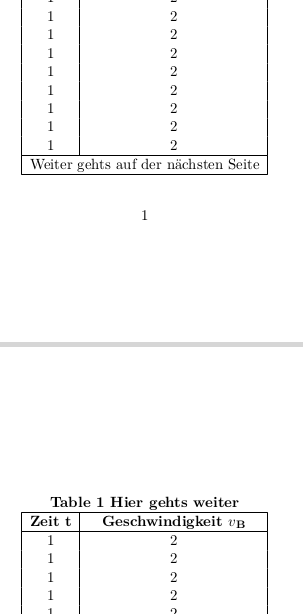
\includegraphics[height=0.8\textheight]{images/longtable_v2.png}
\end{figure}

\end{frame}

\begin{frame}[fragile]
\frametitle{Tabellen über mehrere Seiten}
\framesubtitle{Wichtiges}
\begin{itemize}
\item mit \cmd{endfirsthead} definiert man die oberste Zeile der Tabelle 
\item mit \cmd{endhead} definiert man die oberste Zeile der Tabelle auf den folgenden Seiten
\item mit \cmd{endfoot} und \cmd{endlastfoot} analog die letzten Zeilen
\end{itemize}
\end{frame}



    \uebung{bildertabellen}
    \section{Nützliche Pakete}

\subsection{Einheiten mit \pkg{siunitx}}

\begin{frame}[fragile]
    \frametitle{Einheiten korrekt setzen}
    \framesubtitle{Das Paket \pkg{siunitx}}
    Setzen von Einheiten: \verb+$1.345 V/m$+ \textrightarrow{} $1.345 V/m$
    
    \medskip
    Das sind mindestens 3 typographische Fehler!
    
    \bigskip\pause
    Abhilfe schafft das Paket \pkg{siunitx}:\\
    \verb+\usepackage[locale=DE]{siunitx}+
    
    \medskip\pause
    \begin{block}{Nützliche Optionen}
        \begin{description}
            \item[\texttt{per-mode=symbol}] \SI{1}{\metre\per\second} \textrightarrow{} \SI[per-mode=symbol]{1}{\metre\per\second}
            \item[\texttt{separate-uncertainty=true}] \SI{22 +- 1}{\celsius} \textrightarrow{} \SI[separate-uncertainty=true]{22 +- 1}{\celsius}
    \end{description}
    \end{block}
\end{frame}

\begin{frame}[fragile]
\frametitle{Beispiele}
\framesubtitle{Das Paket \pkg{siunitx}}
    \begin{tabular}{ll}
        \verb+\ang{5}+ & \ang{5}\\
        \verb+\SI{0.587}{kg}+ & \SI{0.587}{kg}\\
        \verb+\SI{9.81}{\metre\per\square\second}+ & \SI{9.81}{\metre\per\square\second}\\
        \verb|\SI{22(1)}{\celsius}| & \SI[separate-uncertainty=true]{22(1)}{\celsius}\\
        \verb|\SI{22 +- 1}{\celsius}| & \SI[separate-uncertainty=true]{22(1)}{\celsius}\\
        \verb+\SI{1,7865e8}{W/(sr.m^2)}+ & \SI{1,7865e8}{W/(sr.m^2)}\\
    \end{tabular}
\end{frame}

\subsection{Einfachere Anführungszeichen}

\begin{frame}[fragile]
    \frametitle{\subsecname}
    \framesubtitle{Das Paket \pkg{csquotes}}
    
    Korrekte Anführungszeichen sind nicht intuitiv:\\
    \verb+"`Hallo"'+ \textrightarrow{} "`Hallo"'
    
    \bigskip\pause
    Abhilfe schafft das Paket \pkg{csquotes}:\\
    \verb+\enquote{Hallo}+ \textrightarrow{} \enquote{Hallo}
    
    \bigskip
    Das Paket verwendet automatisch die korrekten Zeichen, abhängig von der Sprache
\end{frame}
\subsection{Zeilenabstand ändern}

\begin{frame}
    \frametitle{\subsecname}
    \framesubtitle{Das Paket \pkg{setspace}}
    
    Mit dem Paket \pkg{setspace} kann man den Zeilenabstand des Dokuments ändern.

    \bigskip    
    Nach dem Laden kann man den Abstand mit \cmd{doublespacing} oder
    \cmd{onehalfspacing} anpassen
    
    \bigskip
    \begin{block}{Hinweis}
        Dieses Paket ändert nicht den Zeilenabstand in Bildunterschriften oder
        Fußnoten, das sollte auch so gewünscht sein.
    \end{block}
\end{frame}
\subsection{Verlinkungen im Dokument}

\begin{frame}
    \frametitle{\subsecname}
    \framesubtitle{Das Paket \pkg{hyperref}}
    
    Mit dem Laden des Paketes \pkg{hyperref} werden alle Referenzen und Verzeichnisse klickbar, man kann dann sehr einfach zum Ziel des Verweises springen.
    
    \bigskip\pause
    Außerdem kann man mit dem Befehl \cmd{url}\marg{Ziel} eine URL einfügen. Diese ist ebenfalls klickbar.\\
    Beispiel: \url{http://uni-bremen.de}
\end{frame}
\subsection{Ändern der Seitenränder}

\begin{frame}[fragile]
    \frametitle{\subsecname}
    \framesubtitle{Das Paket \pkg{geometry}}
    
    Aufgrund von Vorgaben ist man häufig gezwungen, die Größe der Seitenränder zu ändern.
    
    \medskip\pause
    Dies kann man mit dem Paket \pkg{geometry} erledigen.
    
    \smallskip
    Beispiel: \verb+\usepackage[margin=2cm]{geometry}+
    \smallskip
    
    Dies setzt den Rand überall auf \SI{2}{cm}
\end{frame}
\subsection{Latexmk}

\begin{frame}[fragile]
\frametitle{Latexmk}
\begin{itemize}
  \item Anwendung um das Dokument mit allen Abhängigkeiten zu setzen
  \item Ruft \texttt{pdflatex} solange auf, bis alle Verweise korrekt sind\pause\medskip
  \item In TexLive ist das Programm enthalten
  \item Aufruf über Texmaker (Tools \(\rightarrow\) Latexmk)
  \item Im Texmaker als Standard für Quick Compile wählbar\pause\medskip
  \item Direkt im Terminal mit \verb+latexmk -pdf Datei.tex+
\end{itemize}
\end{frame}
\subsection{Chemische Formeln}

\begin{frame}[fragile]
    \frametitle{\subsecname}
    \framesubtitle{Das Paket \pkg{mhchem}}
    
    Wie auch bei Einheiten ist das korrekte manuelle Setzen chemischer Formeln viel Aufwand.
    
    \medskip\pause
    Daher: Das Paket \pkg{mhchem}. Laden mit:
    \verb+\usepackage[version=3]{mhchem}+
    
    \medskip\pause
    \textbf{Beispiele}\smallskip\\
    \begin{tabular}{ll}
        \verb+\ce{H2O}+ & \ce{H2O}\smallskip\\
        \verb+\ce{Sb2O3}+ & \ce{Sb2O3}\smallskip\\
        \verb|\ce{^227_90Th+}| & \ce{^227_90Th+}\smallskip\\
        \verb|\ce{A <=> B}| & \ce{A <=> B}
    \end{tabular}
\end{frame}
\subsection{Literaturverwaltung}\label{biblatex}

\begin{frame}
    \frametitle{\subsecname}
    \framesubtitle{Das Paket \pkg{biblatex}}
    \begin{itemize}
        \item Biblatex bietet die Möglichkeit Quellenangaben und 
            Literaturverzeichnisse komfortabel zu erstellen.
        \item Benötigte Bibliographie-Datei kann von Literaturverwaltungen exportiert werden
        \item Quellenangabe dann einfach mit \cmd{cite}\marg{Bezeichner}
        \item Quellenverzeichnis mit \cmd{printbibliography}, es werden nur
            benutzte Quellen angezeigt
    \end{itemize}
    
\end{frame}

\uebung{pakete}
    \uebung{pakete}
    \begin{frame}
\frametitle{Die Welt um \LaTeX}
\begin{itemize}
\item Online-Editor mit kompilieren-Funktion \url{Sharelatex.com} und \url{overleaf.com}, eventuell demnächst auch auf Servern der Uni Bremen
\item Lyx (Programm): sieht aus wie Word, macht unten drunter \LaTeX.
\end{itemize}
\end{frame}


    \section{Zeichnen in \LaTeX}
\begin{frame}[fragile]{TikZ ist kein Zeichenprogramm}
\framesubtitle{Das Paket \pkg{tikz}}
Wir wollen nun mit \LaTeX{} ein wenig zeichnen. Dazu laden wir das Paket \pkg{tikz} und bei Bedarf durch \cmd{usetikzlibrary}\marg{Library 1,\dots,Library n} benötigte Bibliotheken für TikZ. 

\medskip\pause
Über die Umgebung \umg{tikzpicture} können wir nun anfangen mit TikZ ein Bild zu zeichnen. Von nun an stehen dem Benutzer eine ganze Reihe Befehle zur Verfügung. Der wichtigste ist hierbei \cmd{draw}\oarg{Options}. 
\end{frame}

\begin{frame}[fragile]{TikZ ist kein Zeichenprogramm}
\begin{block}{Verschiedene Formen}
\begin{tabular}{ll}
\verb+(0,0) -- (0,1)+ & Gerade von (0,0) bis (0,1)\\
\verb+(0,0) circle {r}+ & Kreis mit Radius r um (0,0)\\
\verb+(0,0) rectangle (1,1)+ & Rechteck zwischen (0,0) und (1,1)
\end{tabular}
\end{block}
\begin{block}{Optionen für \cmd{draw}}
\begin{tabular}{ll}
\verb+[->]+ & Kurven und Geraden werden zu Pfeilen\\
\verb+[thick]+ & Kurven und Geraden dick\\
\verb+[dashed]+ & Kurven und Geraden gestrichelt\\
\verb+[fill=red]+ & Inhalt wird rot eingefärbt\\
\end{tabular}\pause

Optionen können auch kombiniert werden. 
\end{block}
\end{frame}

\begin{frame}[fragile]{Beschriftung in TikZ}
\framesubtitle{Der Befehl \cmd{node}}
Wir wollen und können natürlich auch Beschriftungen ergänzen.

\medskip\pause
Der Befehl \cmd{node} ermöglicht dies. Syntax

\begin{center}
\cmd{node}\oarg{Positionierung} \texttt{at} \oarg{Coordinate} \marg{Text}
\end{center}

\medskip\pause
Hierbei genügt auch \cmd{node} \marg{Text} -- Beachte das Leerzeichen! 

\medskip\pause
Positionierung steht dann natürlich für \texttt{above}, \texttt{right}, \texttt{left}, etc. 
\end{frame}

\begin{frame}[fragile]{TikZ ist kein Zeichenprogramm}
\begin{columns}
\begin{column}{0.65\textwidth}
\begin{codeblock}
\begin{small}
\begin{verbatim}
\begin{tikzpicture}[scale=.75]
\draw[thick, rounded corners=8pt,->] 
    (0,0) -- (0,2)
          -- (1,3.25)
          -- (2,2)
          -- (2,0)
          -- (0,2)
          -- (2,2)
          -- (0,0)
          -- (2,0) node[right] 
                  {Das MZH};
\end{tikzpicture}
\end{verbatim}
\end{small}
\end{codeblock}
\end{column}
\begin{column}{0.3\textwidth}
\begin{tikzpicture}[scale=.75]
\draw[thick, rounded corners=8pt,->] (0,0) -- (0,2)
                                           -- (1,3.25)
                                           -- (2,2)
                                           -- (2,0)
                                           -- (0,2)
                                           -- (2,2)
                                           -- (0,0)
                                           -- (2,0) node[right] {Das MZH};
\end{tikzpicture}
\end{column}
\end{columns}
\end{frame}

\begin{frame}[fragile]{Schaltkreise zeichnen}
\framesubtitle{Das Paket \pkg{circuitikz}}
Es besteht unter Umständen das Interesse auch Schaltkreise in \LaTeX\ zu zeichnen. Das geht natürlich auch. Wir benötigen dafür das Paket \pkg{circuitikz} mit der Option \verb|[european]|. Die Syntax ist ähnlich wie bei TikZ.
\begin{columns}
\begin{column}{0.55\textwidth}
\begin{codeblock}
\begin{verbatim}
\begin{circuitikz}
\draw(0,0)
to[battery1, l=$U$] (0,4)
to[ammeter] (2,4)
to[short] (2,0)
to[R] (0,0);
\end{circuitikz}
\end{verbatim}
\end{codeblock}
\end{column}
\begin{column}{0.4\textwidth}
\begin{figure}[h]
\begin{center}
\begin{circuitikz}[scale=0.75]
\draw(0,0)
to[battery1, l=$U$] (0,4)
to[ammeter] (2,4)
to[short] (2,0)
to[R] (0,0);
\end{circuitikz}
\end{center}
\end{figure}
\end{column}
\end{columns}
\end{frame}

\uebung{zeichnen}
    \uebung{zeichnen}
    \begin{frame}
    \begin{center}
    \huge
    Vielen Dank für die Aufmerksamkeit\\\medskip
    und viel Erfolg im ersten Semester!
    \end{center}
\end{frame}

\end{document}
